\documentclass{article}
\usepackage{fancyhdr}
\usepackage{epigraph}
\usepackage{pdfpages}

\pagestyle{fancy}
\fancyhf{}
\lhead{Math 110}
\chead{Project 2}
\rhead{Due: November 4, 2019}
\cfoot{\thepage}


\begin{document}
Salaries can vary greatly depending on your degree, type of
employment, and location; cost of living can also largely vary between
different locations in the world. The goal of this project is to
compare salaries and costs of living in different cities (within the
US). You will complete this project in your assigned groups. Each
group will give a summary presentation to the class; your group will be
graded based on the summary presentation.

\section*{Part 1: Gathering Data}
\begin{enumerate}
	\item Each member of your group should decide what sort of career they want to have as well as a list of three cities in which they may be interested in living.
	\item Using the Occupational Outlook Handbook \newline{\tt https://www.bls.gov/ooh/}, each group member should identify what the national median and average salaries are for your chosen occupation.  Also, look up what each person could expect to earn in your selected cities.
	\item Tax rates vary according to income levels; for purposes of this project, make it easy and assume the total withheld for all taxes is 18\% of the gross salary. Remember that ‘disposable income’ is the amount that remains after taxes. Determine each group member’s ‘disposable income’ based on the median salary in each city.
	\item Using the budgeting guidelines found at \newline{\tt https://www.nomoredebts.org/budgeting-guidelines}, construct a budget for the disposable income which you would realize in each city.
	\item Each group member should investigate the actual cost of
    living in each of their selected cities as well as their home
    town.  Use the cost of living calculator at \newline{\tt https://www.payscale.com/cost-of-living-calculator} to start this investigation.  You may also want to seek out additional resources.  What you will try to do is work out what your life would be like in each city.  Where is the optimal place for you to practice your chosen profession?
\end{enumerate}

\section*{Part 2: Presentation}
Your group will give a 5-10 minute presentation which will include the
following information: 

\begin{itemize}
	\item Salary projections for each group member.
	\item Comparison of the national median and the median in your three selected cities.
	\item Comparison of the budgets you would have in the cities you have chosen based on OOHB data.
	\item Comparison of the cost of living in each of the cities, with special attention being paid to how adequate your income would be for living in each city.  Are any too expensive for you?
	\item A discussion of how your region and profession fit together.  Are there cities that universally pay more, or is it dependent on both variables?
	\item At least three cited sources other than the ones mentioned in this writing prompt.
\end{itemize}

Your presentation must include slides of some sort, either power point
or in some other software.  You will not submit your presentation to
me, rather you will be graded on how well you present the above
information to the class.

Also, attendance is mandatory during the presentation days.  Even if
your group is not presenting, failing to appear on one of these days
without a very good reason will result in a grade of zero for this
project.

Remember, you will be graded as a group. If one group member does not
do their share of the work, it is the responsibility of everyone else
in the group to complete the presentation.  You are accountable to
each other individually, however you are accountable to me
collectively. Moreover, to make this a more realistic simulation, any
group with members who attempt to blame or otherwise betray the other
members will receive a reduced grade. This is, of course, terribly
unfair but this is the way of the world.  Those of you are that are
good workers will be pulling the slothful along with you for the rest
of your lives. This is the real purpose of group projects, to help you
practice coping with that frustration now when the stakes are lower!  

Your presentation will be graded out of 50 points using the
attached rubric. In addition, penalties will be applied for
presentations that are too short or too long, so be sure to practice
and time yourselves.

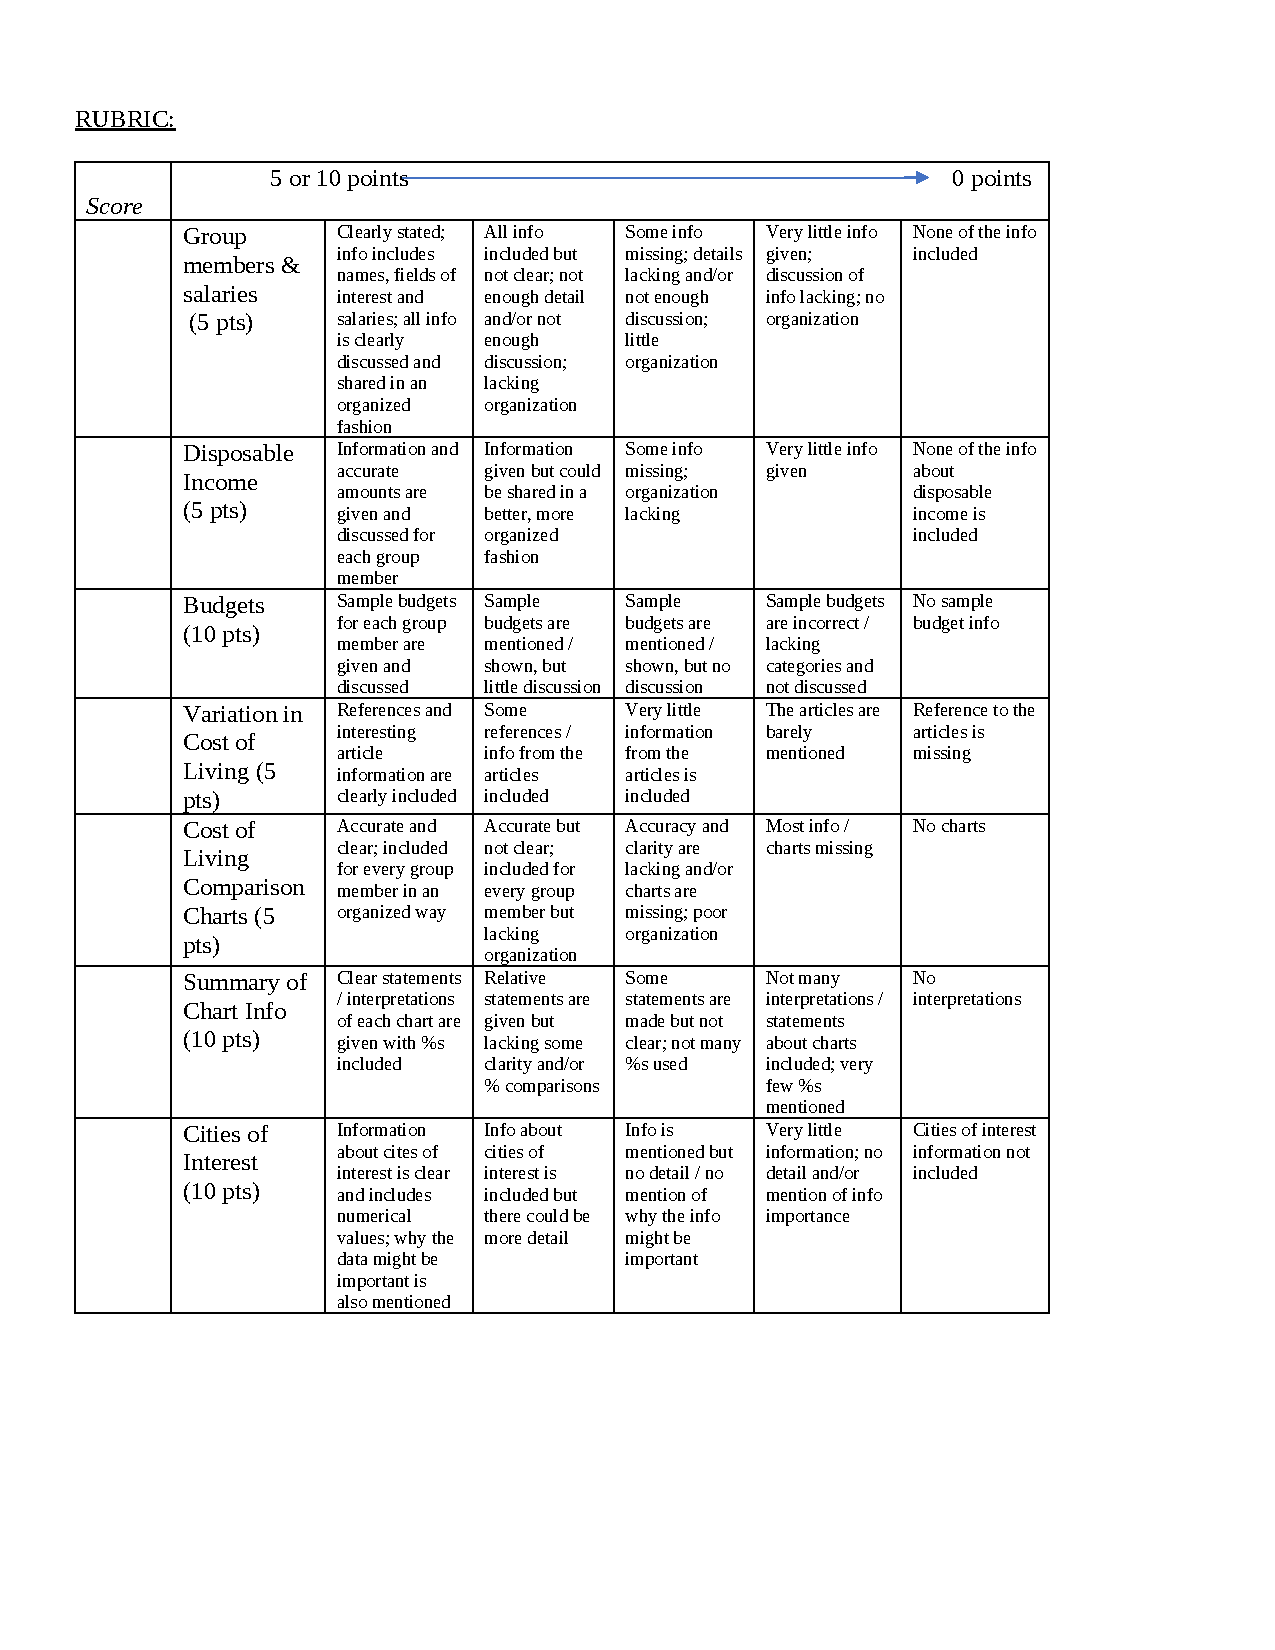
\includepdf[angle=90]{presentation-rubric}
\end{document}
